\section{Introduction}
\label{sec:intro}
\begin{figure*}[!t]
\centering\small
\centering
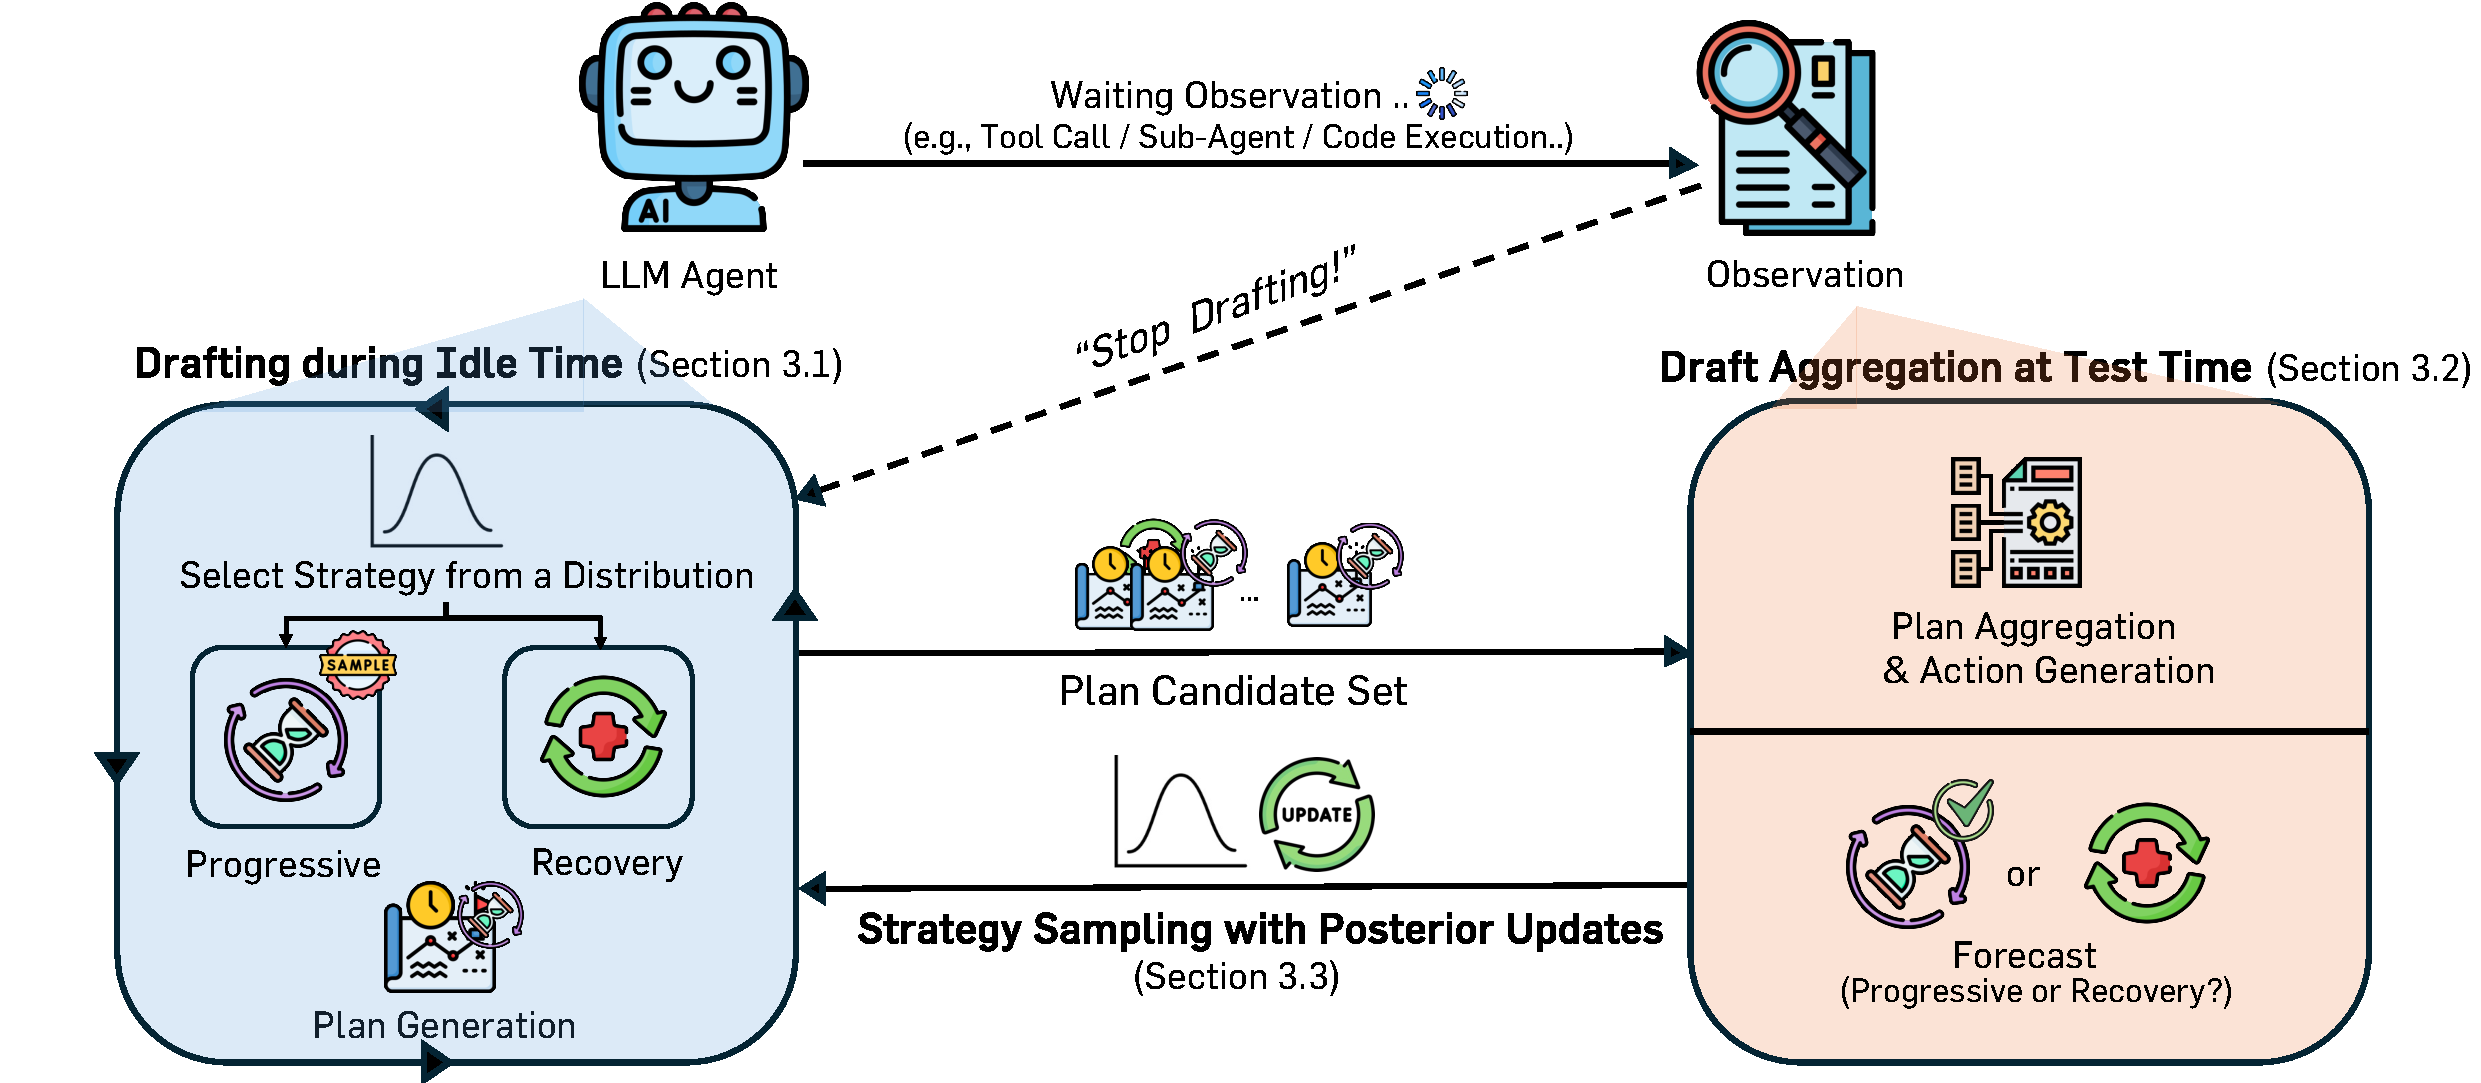
\includegraphics[width=\linewidth,height=0.45\linewidth]{figures/concept_figure.pdf}
\vspace{-2mm}
\caption{
\textbf{Overview of \mname.}
\textbf{(a) Idle-Time Drafting:} during tool execution, the agent iteratively drafts plan candidates by sampling between \textit{Progressive} and \textit{Recovery} strategies, and terminates drafting once the observation arrives.
\textbf{(b) Draft Aggregation:} the agent aggregates the candidates with the observation into a refined action and forecasts whether the trajectory is on track or requires recovery.
\textbf{(c) Posterior Update:} the forecast signal updates the strategy distribution, biasing future drafts toward strategies effective in the current context.
}
\label{fig:concept}
\vspace{-1em}
\end{figure*}

Large language model (LLM)-based agents \cite{yao2022react, sarukkai2025react2} have shown remarkable progress across diverse domains, including general problem solving \cite{mialon2023gaia, phan2025humanity}, web navigation \cite{zhou2023webarena, deng2023mind2web}, code generation \cite{jimenez2023swe, chan2024mle-bench}, and scientific research \cite{lu2024ai}, by actively leveraging external tools such as web search, code interpreters \cite{zhang2024codeagent}, and even other agents \cite{zhang2025agentastool, jiang2025agentadaptation}. Such agents commonly follow a multi-step reasoning loop \cite{yao2022react} in which the agent iteratively reasons, invokes tools, and incorporates the resulting observations, incurring frequent waiting time at each step, referred to as \textit{idle time}. Despite its prevalence in agent execution, the potential of idle time for scaling performance remains largely underexplored, as existing works mainly target efficiency (\eg asynchronously invoking independent tool calls \cite{gim2024async1}). \citet{lin2025sleeptime} first treat idle periods as an opportunity for additional computation that produces auxiliary context, but their design targets LLM–user interactions and remains suboptimal for agentic settings: it ignores variation in tool-call durations, utilizing only 13.7\% of the total idle time on GAIA (see Figure~\ref{fig:gaia-scatter}), and relies on the assumption of predictable future queries, which rarely holds when tool observations are inherently uncertain, often degrading performance (see \textit{Sleep-time Compute} in Table~\ref{tab:main1}).




This raises a key question:
\textit{How can we develop a robust, generalizable solution for exploiting idle time arising from agentic interactions to improve agent performance on complex tasks?
} This naturally leads us to analyze idle time across diverse agentic scenarios and explore effective strategies for leveraging it. Our analysis yields the following key observations: 

\begin{itemize}
\item \textit{Reasoning budgets for idle time are substantial but highly variable across tool calls.} 
We observe that the available reasoning budget during idle time is sufficiently large across diverse benchmarks---including tool-augmented reasoning (GAIA), multi-hop search (FRAMES), and execution-heavy environments (MLE-Bench)---providing additional computation to improve performance. However, the amount of available budget varies significantly across individual tool calls.


\item \textit{Planning is more effective than other agent strategies during idle time.} 
Among representative agent strategies, \ie summarization, reflection, and planning, we find that planning yields the most consistent performance improvements when generated during idle time.
\end{itemize}

Motivated by these findings, we propose \lname, a scalable inference framework that exploits idle time via speculative planning; see the overview in Figure~\ref{fig:concept}. Specifically, we adopt a simple yet effective two-phase strategy: (a) during idle time, the agent iteratively generates candidate plans; (b) once observations arrive, these candidates are aggregated and conditioned to guide subsequent reasoning. For higher utilization of idle time, the agent iteratively drafts candidates until an observation becomes available and terminates immediately upon observation arrival, thereby enabling higher utilization of idle time. 


The key challenge of planning during idle time lies in handling observation uncertainty.
Since observations are not yet available during idle periods, generated plans may become invalid or suboptimal once the observation becomes available.
To mitigate this uncertainty, we design a drafting strategy distribution that dynamically samples between two complementary strategies: \textit{Progressive}, which assumes favorable observations and emphasizes exploitation, and \textit{Recovery}, which explores alternative solution paths assuming potential failure from observation. 
By generating both forward-progressing and recovery-oriented drafts through sampling, the agent improves coverage over plausible future observations.
Furthermore, this strategy distribution is updated via posterior feedback, whereby the agent evaluates its current progress and forecasts the most suitable drafting strategy for subsequent idle periods. This adaptive update enables the drafting behavior to be adjusted during inference, resulting in robust performance across diverse execution contexts.

To validate the effectiveness and generality of \mname, we conduct extensive experiments across three diverse agentic benchmarks: tool-augmented reasoning, multi-hop search, and long-horizon interactive tasks.
We first evaluate \mname on the GAIA benchmark \cite{mialon2023gaia}, which requires diverse capabilities including web search, file inspection, and code execution, and on FRAMES~\cite{krishna2024frames}, which requires multi-hop search via repeated agent-as-tool invocations.
We show that \mname consistently improves performance across various LLM backbones, \eg surpassing the vanilla baseline by 4.6\% and 6.8\% in average accuracy on Gemma4-E4B and Qwen3.5-4B, respectively. The performance gains are also more consistent than those of prior idle-time approaches \cite{lin2025sleeptime}, which exhibit lower utilization of total idle time and, in some cases, even degrade baseline performance. 
Next, we verify the generality of \mname on MLE-Bench \cite{chan2024mle-bench}, a benchmark that involves substantial idle time due to code execution for machine learning engineering scripts. In this setting, \mname significantly outperforms all baselines, highlighting its applicability to complex, long-horizon interactive tasks.

\textbf{Contributions.}
Our contributions are as follows:
\begin{itemize}
    \item We conduct a systematic analysis of idle time in LLM-based agents across diverse agentic scenarios, showing that idle periods are substantial but vary significantly across tool calls. We further establish that planning yields more effective use of idle-time computation than other agentic strategies such as summarization and reflection.
    
    \item We propose \mname, a scalable inference-time framework that exploits idle time in agentic interactions via speculative planning. 
    \mname iteratively and adaptively generates candidate plans by sampling from a strategy distribution, and aggregates them once the observations for the next step become available. 
    
    \item We validate \mname across three diverse agentic benchmarks, \ie GAIA, FRAMES, and MLE-Bench, spanning tool-augmented reasoning, multi-hop search, and long-horizon interactive tasks, and demonstrate consistent performance gains over existing baselines. 
\end{itemize}



